\section{Zweitore - Vierpoltheorie}
\subsection{Zweitorgleichungen}
% \includegraphics[width=\columnwidth]{Zweitorgleichungen}
\begin{mdframed}[style=exercise]
    \begin{itemize}
        \item{Admittanzform/ Admittanzmatrix \textbf{Y}:}
        \begin{align*}
            \begin{split}
                \underline{I}_1 &= \underline{Y}_{11}\cdot\underline{U}_1 + \underline{Y}_{12}\cdot\underline{U}_2\\
                \underline{I}_2 &= \underline{Y}_{21}\cdot\underline{U}_1 + \underline{Y}_{22}\cdot\underline{U}_2
            \end{split}
        \left\} \
            \begin{pmatrix}
                \underline{I}_1 \\
                \underline{I}_2
            \end{pmatrix} = \textbf{\underline{Y}}\cdot
            \begin{pmatrix}
                \underline{U}_1 \\
                \underline{U}_2
            \end{pmatrix}
        \right.
        \end{align*}
        \item{Impedanzform/ Impedanzmatrix \textbf{Z}:}
            \begin{align*}
                \begin{split}
                \underline{U}_1 &=\underline{Z}_{11}\cdot\underline{I}_1 + \underline{Z}_{12}\cdot\underline{I}_2 \\
                \underline{U_2} &=\underline{Z}_{21}\cdot\underline{I}_1 + \underline{Z}_{22}\cdot\underline{I}_2
                \end{split}
            \left\} \
                \begin{pmatrix}
                    \underline{U}_1 \\
                    \underline{U}_2
                \end{pmatrix} = \textbf{\underline{Z}}\cdot
                \begin{pmatrix}
                    \underline{I}_1 \\
                    \underline{I}_2
                \end{pmatrix}
            \right.
            \end{align*}
        \item{Hybridform 1/ Reihenparallelmatrix \textbf{H}:}
            \begin{align*}
                \begin{split}
                    \underline{U}_1 &= \underline{H}_{11}\cdot\underline{I}_1 + \underline{H}_{12}\cdot\underline{U}_2 \\
                    \underline{I}_2 &= \underline{H}_{21}\cdot\underline{I}_1 + \underline{H}_{22}\cdot\underline{U}_2
                \end{split}
            \left\} \
                \begin{pmatrix}
                    \underline{U}_1 \\
                    \underline{I}_2
                \end{pmatrix} = \textbf{\underline{H}}\cdot
                \begin{pmatrix}
                    \underline{I}_1 \\
                    \underline{U}_2
                \end{pmatrix}
            \right.
            \end{align*}
            \item{Hybridform 2/ Parallelreihenmatrix \textbf{C}:}
            \begin{align*}
                \begin{split}
                    \underline{I}_1 &= \underline{C}_{11}\cdot\underline{U}_1 + \underline{C}_{12}\cdot\underline{I}_2 \\
                    \underline{U}_2 &= \underline{C}_{21}\cdot\underline{U}_1 + \underline{C}_{22}\cdot\underline{I}_2
                \end{split}
            \left\} \
                \begin{pmatrix}
                    \underline{I}_1 \\
                    \underline{U}_2
                \end{pmatrix} = \textbf{\underline{C}}\cdot
                \begin{pmatrix}
                    \underline{U}_1 \\
                    \underline{I}_2
                \end{pmatrix}
            \right.
            \end{align*}
            \item{Kettenform/ Kettenmatrix \textbf{A}:}
                \begin{align*}
                    \begin{split}
                        \underline{U}_1 &= \underline{A}_{11}\cdot\underline{U}_2 + \underline{A}_{12}\cdot-\underline{I}_2 \\
                        \underline{I}_1 &= \underline{A}_{21}\cdot\underline{U}_2 + \underline{A}_{22}\cdot-\underline{I}_2
                    \end{split}
                \left\} \
                    \begin{pmatrix}
                        \underline{U}_1 \\
                        \underline{I}_2
                    \end{pmatrix} = \textbf{\underline{A}}\cdot
                    \begin{pmatrix}
                        \underline{U}_2 \\
                        -\underline{I}_2
                    \end{pmatrix}
                \right.
                \end{align*}
                \item{Kettenform rückwärts/ Kettenmatrix \textbf{B}:}
                    \begin{align*}
                        \begin{split}
                            \underline{U}_2 &= \underline{B}_{11}\cdot\underline{U}_1 + \underline{B}_{12}\cdot-\underline{I}_1\\
                            \underline{I}_2 &= \underline{B}_{21}\cdot\underline{U}_1 + \underline{B}_{22}\cdot-\underline{I}_1
                        \end{split}
                    \left\} \
                    \begin{pmatrix}
                        \underline{U}_2\\
                        \underline{I}_2
                    \end{pmatrix} = \textbf{\underline{B}}\cdot
                    \begin{pmatrix}
                        \underline{U}_1 \\
                        -\underline{I}_1
                    \end{pmatrix}
                \right.
                    \end{align*}
    \end{itemize}
\end{mdframed}

\subsubsection{Parameterumrechnung}
% \begin{table}[htbp]
%     \begin{tabular}{c|c|c|c|c|c}
%         $Z$ & $Y$ & $H$ & $A$ & $C$\\
%         \hline
%         $
%         \begin{bmatrix}
%             \underline{Z_11} & \underline{Z_12}\\
%             \underline{Z_21} & \underline{Z_22}
%         \end{bmatrix}
%         $
%         &$
%             \begin{bmatrix}
%                 \dfrac{\underline{{Y}_{22}}}{\operatorname{det}\underline{\boldsymbol{Y}}} & \dfrac{-\underline{Y}_{12}}{\operatorname{det} \underline{\boldsymbol{Y}}}\\
%                 \dfrac{-\underline{Y}_{21}}{\operatorname{det} \underline{\boldsymbol{Y}}} & \dfrac{\underline{{Y}}_{11}}{\operatorname{det} \underline{\boldsymbol{Y}}} \\
%             \end{bmatrix}
%         $  & a & n\\
%     \end{tabular}
% \end{table}
\includegraphics[width=\columnwidth,height=9cm]{Parameterumrechnung}\\
% \newpage0\newpage \onecolumn

\subsection{Zusammenschalten von Zweitoren}

\begin{mdframed}[style=exercise]
\begin{itemize}
    \item Reihenschaltung:
        \begin{center}
            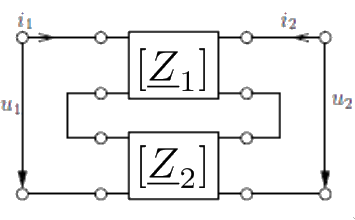
\includegraphics[width=0.5\textwidth]{Reihenschaltung_Zweitore}
        \[
            \left[ \underline{Z} \right] = \left[ \underline{Z}_1 \right] + \left[ \underline{Z}_2 \right]
        \]
        \end{center}
    \item Parallelschaltung:
        \begin{center}
            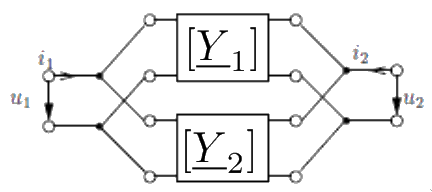
\includegraphics[width=0.6\textwidth]{Parallelschaltung_Zweitoren}
        \[
            \left[ \underline{Y} \right] = \left[ \underline{Y}_1 \right] + \left[ \underline{Y}_2 \right]
        \]
        \end{center}
    \item Kettenschaltung:
        \begin{center}
            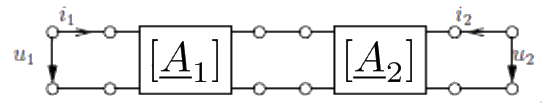
\includegraphics[width=0.7\textwidth]{Kettenschaltung_Zweitoren}
        \[
            \left[ \underline{A} \right] = \left[ \underline{A}_1 \right] \cdot \left[ \underline{A}_2 \right]
        \]
        \end{center}
        \footnotesize
        \textsc{Beachte:}\\
        \normalsize Im Allgemeinen gilt $\rightarrow
        \left[ \underline{A}_1 \right] \cdot \left[
        \underline{A}_2 \right] \neq \left[ \underline{A}_2
        \right] \cdot \left[ \underline{A}_1 \right]$
    \item Reihen-Parallelschaltung:
        \begin{center}
            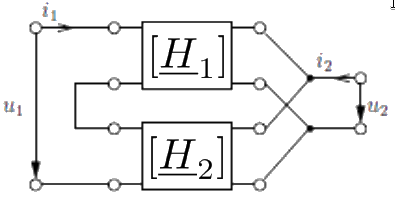
\includegraphics[width=0.5\textwidth]{Reihen-Parallelschaltung_Zweitoren}
        \[
            \left[ \underline{H} \right] = \left[ \underline{H}_1 \right] \cdot \left[ \underline{H}_2 \right]
        \]
        \end{center}
    \item Parallel-Reihenschaltung:
        \begin{center}
            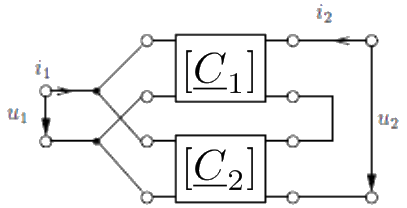
\includegraphics[width=0.5\textwidth]{Parallel-Reihenschaltung_Zweitoren}
        \[
            \left[ \underline{C} \right] = \left[ \underline{C}_1 \right] \cdot \left[ \underline{C}_2 \right]
        \]
        \end{center}
\end{itemize}
\end{mdframed}


\begin{samepage}
    \onecolumn
    \subsection{Matrizen elementarer Zweitore}
    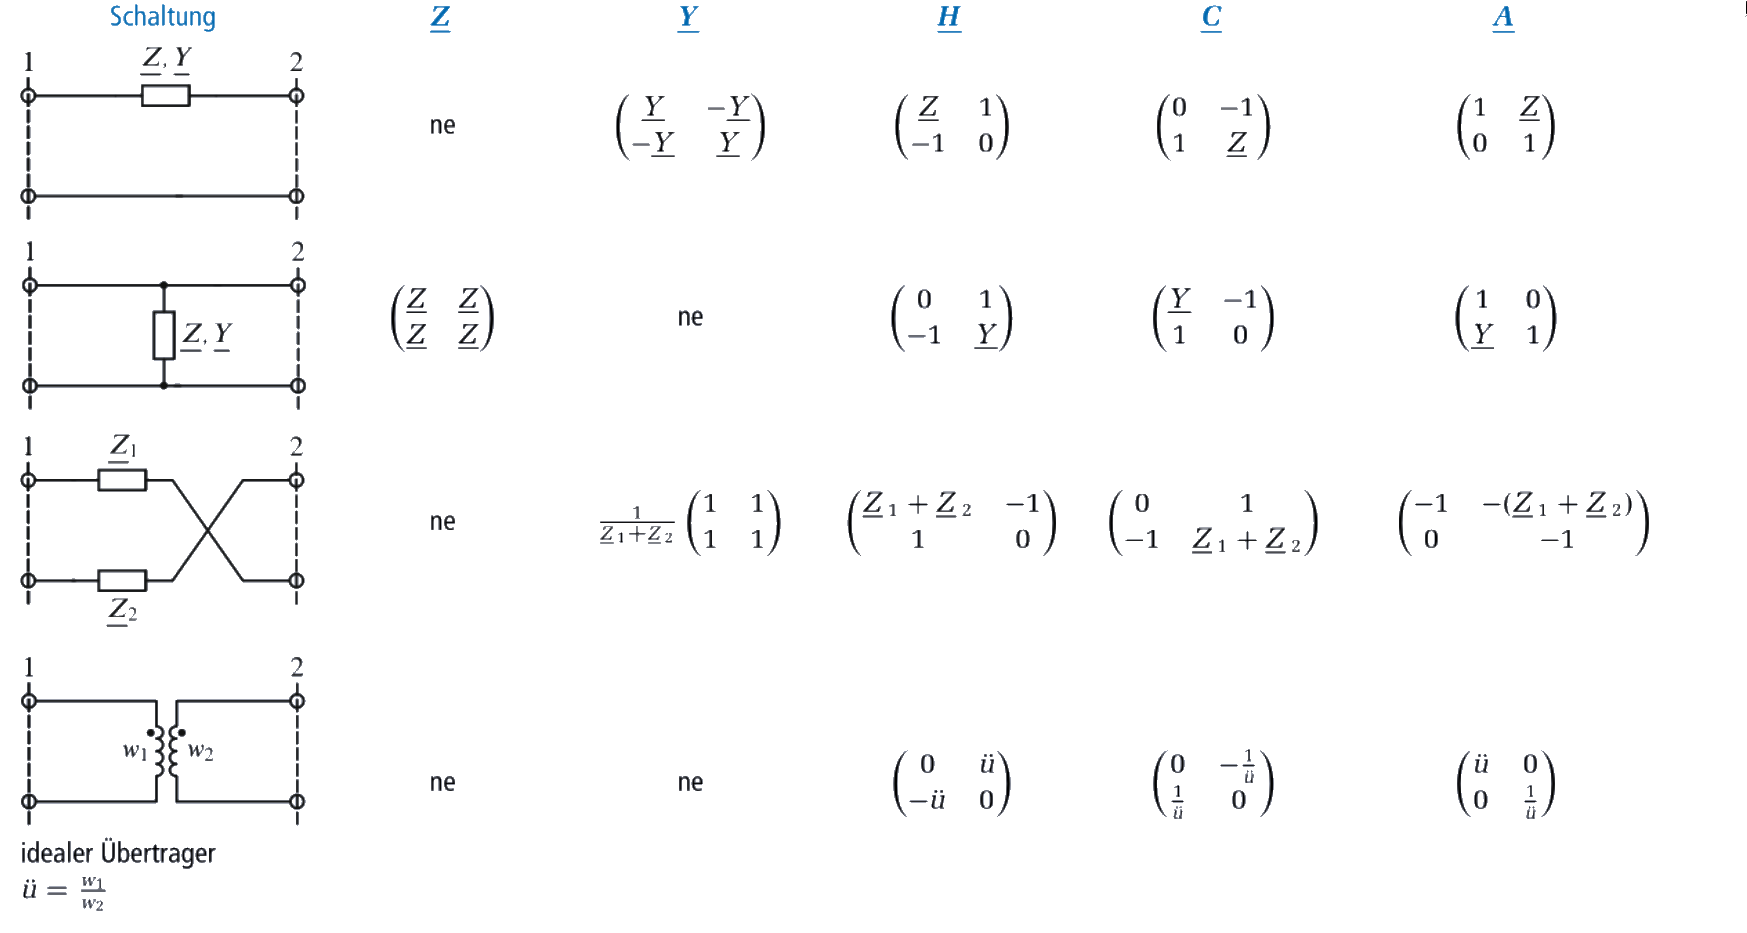
\includegraphics[width=\columnwidth]{converted/Matrizen_elementarer_zweitore}
    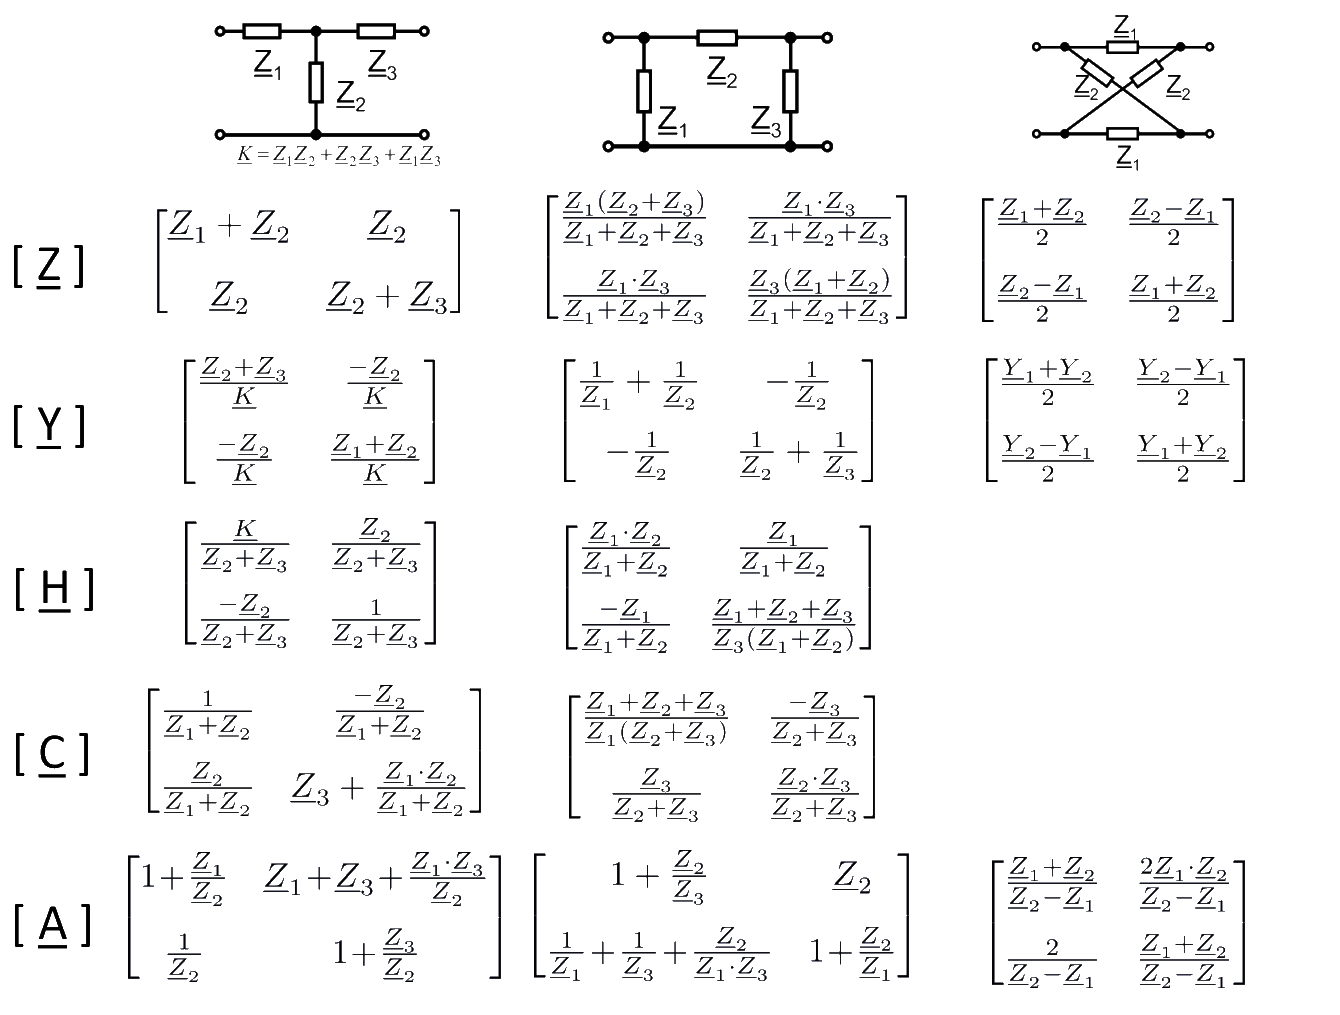
\includegraphics[width=\columnwidth]{converted/Matrizen_elementarer_zweitore_1}
\end{samepage}
\twocolumn

\subsection{Torbedingungen}
